\section{Introduction}

\begin{figure*}[t]
    \centering
    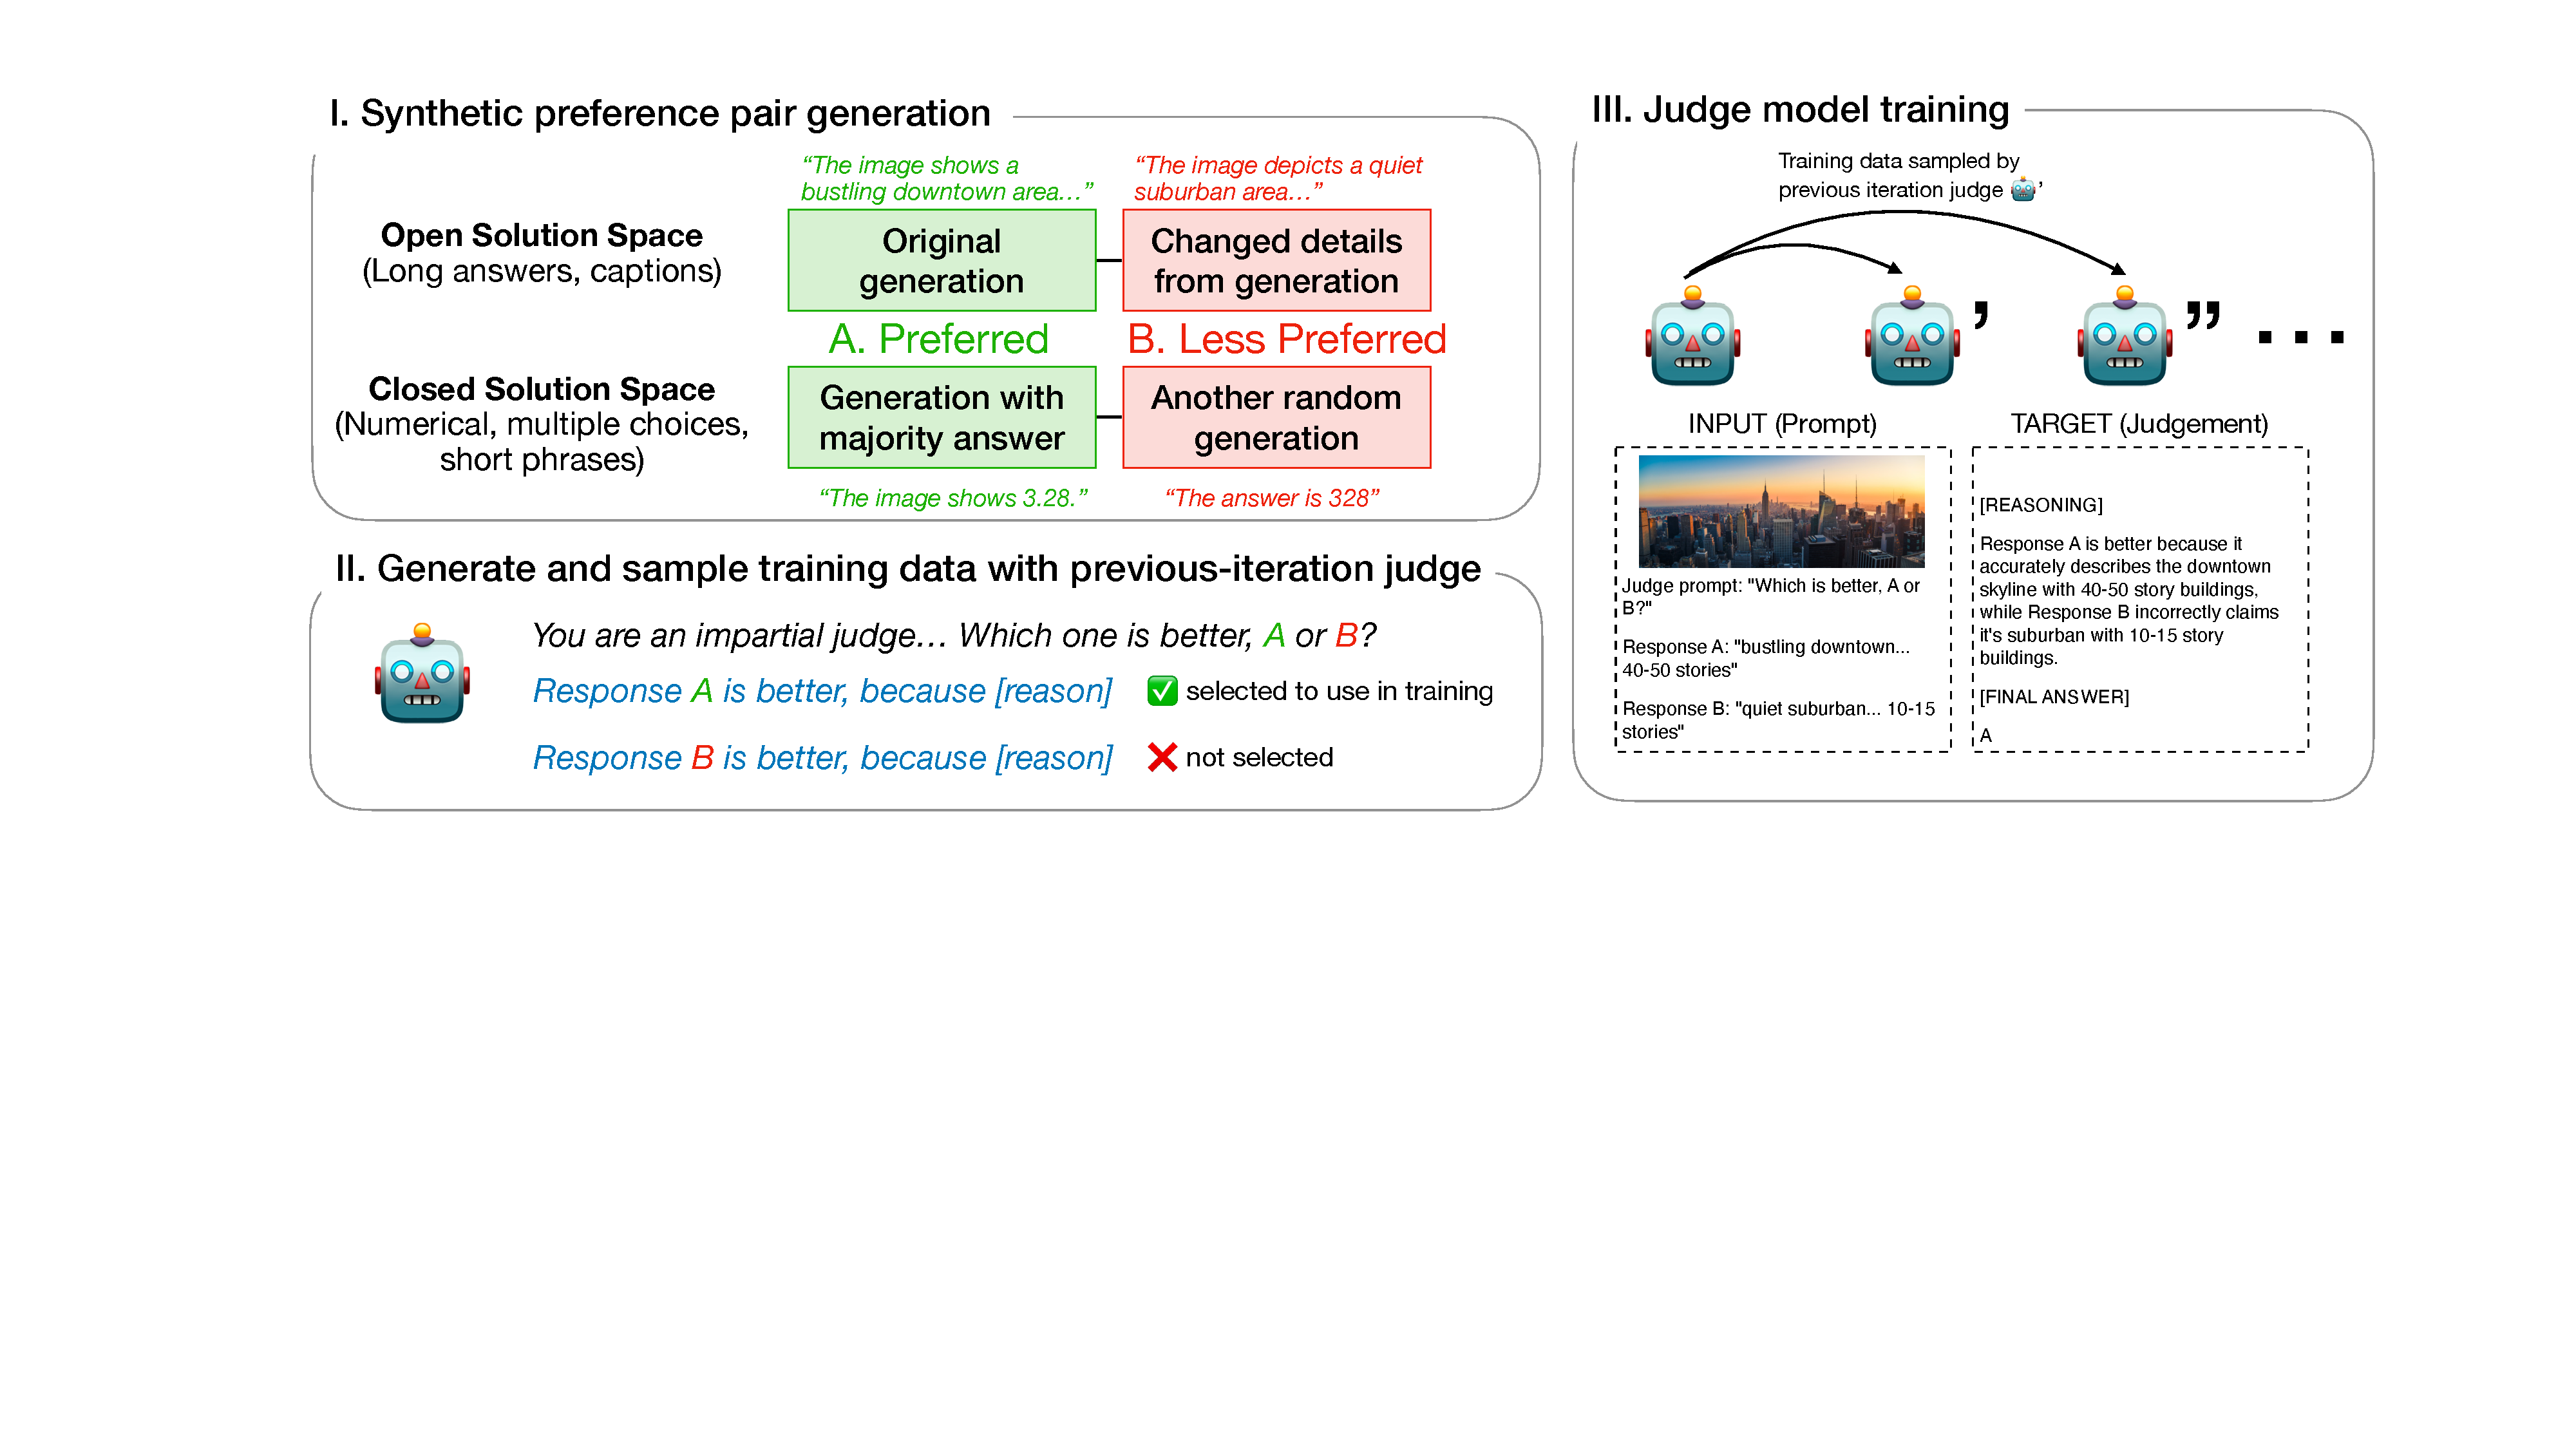
\includegraphics[width=\textwidth,trim={5cm 16cm 5cm 0cm}, clip]{images/fig1.pdf}
    \caption{Self-improving VLM judge:  iterative synthetic preference data generation and judge model fine-tuning pipeline. \textbf{I. Synthetic preference pair generation.} We create synthetic preference pairs tailored to different question types. For open solution space questions (long answers, captions), we generate an original response and deliberately inject meaningful errors to create a less preferred version. For closed solution space questions (numerical, multiple choice, short phrases), we generate multiple candidates and pair the majority answer with a random alternative. \textbf{II. Iterative judge training data generation.} We use the previous-iteration judge model to evaluate the newly synthesized preference pairs and gather the judge's reasoning traces. We retain only judgments that align with our synthetic preferences. \textbf{III. Judge model training.} We fine-tune the previous-iteration judge model on these filtered reasoning traces. We iterate this three-step process several times. More details in \S\ref{sec:method}.}
\end{figure*}



VLM reward models are critical for evaluating output quality and enabling alignment with human preferences~\cite{yu2025rlaif, jing2024fgaif,2023llavarlhf, chen2024mllm}.

Existing approaches for training such model evaluators have primarily followed two directions: scaling up human preference collection and distilling from large closed-source models such as GPT and Claude (which also indirectly rely on significant human annotation)~\cite{li2024vlfeedback, llava-critic, zhang2023gpt4vevaluator, povid}. 
However, extensive human preference annotation is both costly and labor-intensive, and becomes obsolete as models advance and new tasks arise. 

In this paper, we show that it is possible to self train a VLM judge given only the VLM's own generations. 

Our method requires no human preference annotations, thereby significantly reducing the cost of reward model training. 

The key idea is that it is possible to use simple, general purpose heuristics to find or construct VLM outputs with varied quality levels, which provide enough signal to train a judge.  Our approach follows a three-step iterative process:
\begin{itemize}[noitemsep,topsep=0pt,leftmargin=*]
  \item \textbf{Synthetic preference pair generation.} We create synthetic preference pairs tailored to different question types. For questions with closed-ended answers (e.g. multiple choice or numerical problems) we generate many candidate responses and pair the majority answer with a random alternative. For open-ended questions (e.g. like captioning) we generate responses and deliberately inject meaningful errors into one version, such as changing object attributes or spatial relationships. We create substantial differences rather than minor edits, exposing the model to realistic evaluation scenarios.
  \item \textbf{Judge training data generation.} 
 
We use the previous-iteration judge model to evaluate the newly synthesized preference pairs and gather the judge's answer and reasoning traces.
Since we know the preferred pair by construction, we retain only judgments that align with our synthetic preferences.
  \item \textbf{Judge model training.} We fine-tune the previous-iteration judge model on these filtered reasoning traces and answers. 
\end{itemize}
We iterate this three-step process several times. We iteratively train a small Llama-3.2-11B model~\cite{llama3} using our framework, and evaluate the model with VL-RewardBench~\cite{vlrb} and Multimodal RewardBench~\cite{mmrb}. Our method improves the model from 0.38 to 0.51 overall accuracy, often outperforming much larger models like Llama-3.2-90B and Claude 3.5 Sonnet~\cite{claude} on VL-RewardBench.
In Section~\ref{sec:analysis}, we systematically analyze the impact of synthetic data design and iterative refinement, providing insights into the conditions under which self-improvement is most effective for VLM judge training. 
Specifically, our synthetic data construction provides a way to create a preference dataset from any visual queries, even without any reference answers.
This makes our framework applicable to new visual tasks where ground-truth annotations are unavailable or scarce, such as evaluating responses to novel image collections or emerging visual domains. Overall, our contributions include:
\begin{itemize}[noitemsep,topsep=0pt,leftmargin=*]
    \item A method to create diverse synthetic preference data for VLMs without human preference annotations, using majority voting consensus for closed-ended tasks and controlled error injection for open-ended tasks.
    
    \item An iterative self-improvement framework that trains VLM judges by filtering and learning from self-generated reasoning traces, enabling iterative refinement of evaluation capabilities.
    
    \item Empirical demonstration that our approach enables a compact 11B model to gain substantial improvements on several reward benchmarks, even surpass much larger models (90B) and proprietary systems (Claude 3.5 Sonnet) on VL-RewardBench.
    
    \item Analysis showing scaling trend over increasing iterations, and operates effectively without access to ground-truth answers, making it applicable to emerging visual domains where annotations are scarce or unavailable.
\end{itemize}

